\section{Proposed Solution}
We propose a solution which can convert a Java class file to a UPPAAL SMC model, rewrite it to insert fault injection attack countermeasures and recommend one of these countermeasures. The point of the conversion to a model, is to be able to provide guarantees about certain properties of the program. This makes sense when the Java class file is rewritten and countermeasures are inserted, since it is then possible to guarantee that the program has not become less secure with respect to certain properties.\\

The workflow stages of the solution are illustrated in \cref{fig:workflow}. The stages are labelled with numbers 1-5. Their purposes are detailed in the following.

% burde vi ogs� give mulighed i programmet for bare at f� en ``vanilla'' SMC model ud?

\paragraph{Stage 1 - 3} parses Java bytecode code through the solution's parser and generates a UPPAAL SMC model.
\paragraph{Stage 2 - 3} parses Java bytecode code, modified with fault countermeasures, through the solution's parser and generates a UPPAAL SMC model.  
\paragraph{Stage 3 - 4} assesses the performed attacks and countermeasures implemented to reduce vulnerablility, by verifying properties about them.
\begin{figure}[H]
\centering
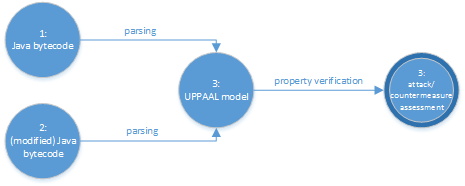
\includegraphics[width=1\textwidth]{figures/workflow_new.png}
\caption{The workflow of the solution, from Java bytecode to UPPAAL SMC model}
\label{fig:workflow_new}
\end{figure}
\ch{should we go from java source to ... or from java bytecode to.. in either case, adjust both figures to start from the same "place"}